\documentclass[12pt]{article}
\usepackage{graphicx}
\usepackage[margin=0.75in]{geometry}
\usepackage{wrapfig}
\usepackage{hyperref}
\usepackage{float}
\usepackage{parskip}
\setlength{\parskip}{1em}

\begin{document}

\title{Security Vulnerabilities in Open Source Electronic Design Automation Software}
\author{Weston Braun}
\maketitle

\section{Introduction}
\label{S:1}
With the rise of the new ``Maker'' movement the number of open source software projects hosted online has rapidly risen. Work on these open source projects includes the wide exchange of files for electronic design automation (EDA) software, often from semi-anonymous users. The goal of this project is to take a analyze some EDA programs and see if this behavior represents a so far overlooked security risk. 

\section{Threat Model}
\label{S:2}
Open Source implies that the design files and code of a open source hardware project are publicly hosted. A typical hardware project consists of a schematic with its associated printed circuit board (PCB) layout, code for a microcontroller, and possibly 3D CAD files for an enclosure. Due to the crossover between the open source hardware and open source software communities, git is commonly used for version control with hosting through github or similar services. Project discovery happens though aggregator websites such as hackaday.com or dangerousprototypes.com, mailing lists, publications such as Make Magazine, or through search engines. 

Once a user discovers a project they are often interested in viewing the schematic and PCB layout. To do so they need to download the project files and open them on their computer. Unlike a software project where a makefile can be viewed in a text editor before running any commands, or code that can be reviewed before being compiled, most EDA file formats are not optimized for direct user readability. Often, the only way to view the hardware design files is through the same EDA software that the project developer used. Cross compatibility between different EDA programs is uncommon. 

The origins of many of these open source EDA programs date back to a time when public hosting of projects was less common and the viewing and modification of files from the internet at large was not a central use case. However, with the current open source hardware community, this is now common, if not expected, behavior. It is believed that the difference between the original design philosophy of the software and the current usage leaves an appreciable attack surface the may be used to target the end user.  

As an additional threat, some PCB manufactures targeted towards the hobby and open source community have begun directly accepting EDA software files instead of the industry standard gerber files, which are a direct numerical representation of the PCB traces and holes. On the manufacturer's server an instance of the EDA program will generate the gerber files which are then used for production. This presents an additional attack surface where an exploit in an EDA program could be leveraged against a commercial service. 


\section{Target Software}
\label{S:3}
Popular EDA software used in the open source hardware community includes KiCad, Eagle, Altium, and gEDA. These programs all feature relatively the same work flow. They consist of a schematic capture tool where the user creates an electrical schematic using a library of component symbols. There is an association between the schematic symbols and physical part footprints which the user uses to create a PCB design. 

Of the programs mentioned, both KiCad and gEDA are open source with KiCad written in C++ and gEDA written in C. In each of these programs the schematic capture tool and PCB layout tool are isolated as independent executables. KiCad is currently the more popular program with development funding being provided by CERN. However, both are available through the Debian repositories with gEDA using the package name `pcb' and kicad using the package name `kicad'. Early analysis was conducted on both programs with the focus shifting to gEDA based on findings. 


\section{Vulnerability Search}
\label{S:4}
Because of the previously mentioned threat model of manufacture accepted PCB layout files, the search for vulnerabilities focused on the pcb layout component of KiCad and gEDA. The search for vulnerabilities consisted of manual code review aided by static analysis and then fuzzing. The biggest attack surface was expected to be the parsers, which parses the text based PCB layout and netlist, consisting of part names, locations, and pin connections, into a data structure for display and modification. A vulnerability in the parser would allow for an exploit to execute through the user opening the file without any additional action. An additional attack surface discovered in this process was the user interface itself. Malicious strings can make it through the parser and exploit display formatting functions. 

\subsection{Static Analysis / Code Review}
KiCad and gEDA both have significant code bases, consisting of a parser for file input, functions to modify the schematic or PCB, and the GUI. According to the CLOC utility, the KiCad PCB utility, pcbnew, has a codebase of 109,386 lines of C++ code while the codebase for the gEDA PCB utility, pcb, has 102,379 lines of C code. This size of this codebase makes full manual review difficult. A static analysis tool, which searches through the code for potentially unsafe functions or pointer arithmetic, was used to reduce the scope of this search. Flawfinder, a utility available in the Debian package manager, is capable of parsing C and C++ code and proved suitable for this purpose. 

Running on the KiCad pcbnew codebase, Flawfinder yielded 104 potential security vulnerabilities. Upon manual review of these hits it was revealed that as a class of vulnerabilities, string based buffer overflows were in large prevented through the consistent use of the wxString library, which dynamically resizes strings to preventing buffer overflows. There were some potentially interesting issues relating to race conditions on file access. However, they are not applicable to the threat model of exploitation via a malicious file. Due to the more modern and better maintained codebase and use of C++ features that make buffer overflows more difficult it was decided at this point that gEDA would present a more promising target. 

When run on the gEDA pcb codebase Flawfinder yielded 487 potential security vulnerabilities. Upon review of these hits two buffer overflows relating to the pin display names were discovered. Both of these are triggered by user action through the GUI. One is a heap overflow triggered by the user moving the mouse over a pin. This pops up a dialog box showing the pin name and number, allowing for an overflow of the buffer for the pin number. A stack overflow is achievable through the formatting function of the pin number for the dialog box used by the change pin name tool. Flawfinder outputs and commentary are available on the project github repo. 

\subsection{Fuzzing}
\subsubsection{Implementation} 
Fuzzing was used with the hope of finding exploitable errors in the gEDA pcb parser. The fuzzer of choice, AFL-fuzz, requires an instrumented binary compiled afl-gcc that will terminate on its own as well as one or more minimal input files to use as a basis for fuzzing. An example PCB layout was reduced down to a minimal feature set and the gEDA pcb source was modified to terminate after parsing the input file. Initial fuzzing attempts on a test VM were very slow (4 executions per second) due to CPU limitations and the GUI launching with every execution. Attempts were made to separate the parsing functions from the GUI to speed up execution but the parsing functions required the memory structures initialized by the GUI library. Bypassing this would have required a rewrite of part of the GUI library which was deemed beyond the scope of the project. Using a dedicated machine with a fake x11 display driver improved performance and allowed for approximately 100 executions per second. The fuzzing was allowed to run for 24 hours to achieve acceptable path coverage. 

\subsubsection{Results}
Fuzzing yielded 340 unique crashes. This ended up being significantly more files than were practical to review within the time constraints of the project. A random subset of the files were manually with reviewed and analyzed with gdb. This revealed a significant number of heap corruption errors, some segfaults, and a stack overflow. It was discovered that with the heap corruption errors the final crash was occurring when the PCB memory structure was freed which occurred significantly after the original out of bounds write in the heap. Valgrind was used to profile the program when parsing these files and discover the actually line of code causing the heap corruption.


The most interesting errors that were discovered via fuzzing were a stack overflow and an out of bounds memory write that could possibly be controlled to overwrite arbitrary locations in memory. The stack overflow is triggered though incorrectly formatted PCB trace descriptions causing the parser function to iterate out of array bounds. The out of bounds memory write is is triggered through incorrectly formatted pcb layer descriptions causing a parsing error and receiving an out of bounds index, leading the writing of the layer number out of bounds. Analysis of more vulnerabilities discovered by the parser is hosted on the projects github page.  

\section{Exploit}
\label{S:5}
Even though none of the discovered vulnerabilities would have allowed for the creation of an exploit that would work against the version of the gEDA pcb program available from the package manger it was decided that a proof of concept exploit should be developed that could run against an unmodified codebase but with the standard protections disabled. For this exploit the stack based buffer overflow of the pin display number discovered via static analysis was chosen as the base vulnerability. This stack overflow is triggered through the dialog box for changing the pin name, which is shown in Figure \ref{fig:rename-gui}. 
\begin{figure}[H]
\centering
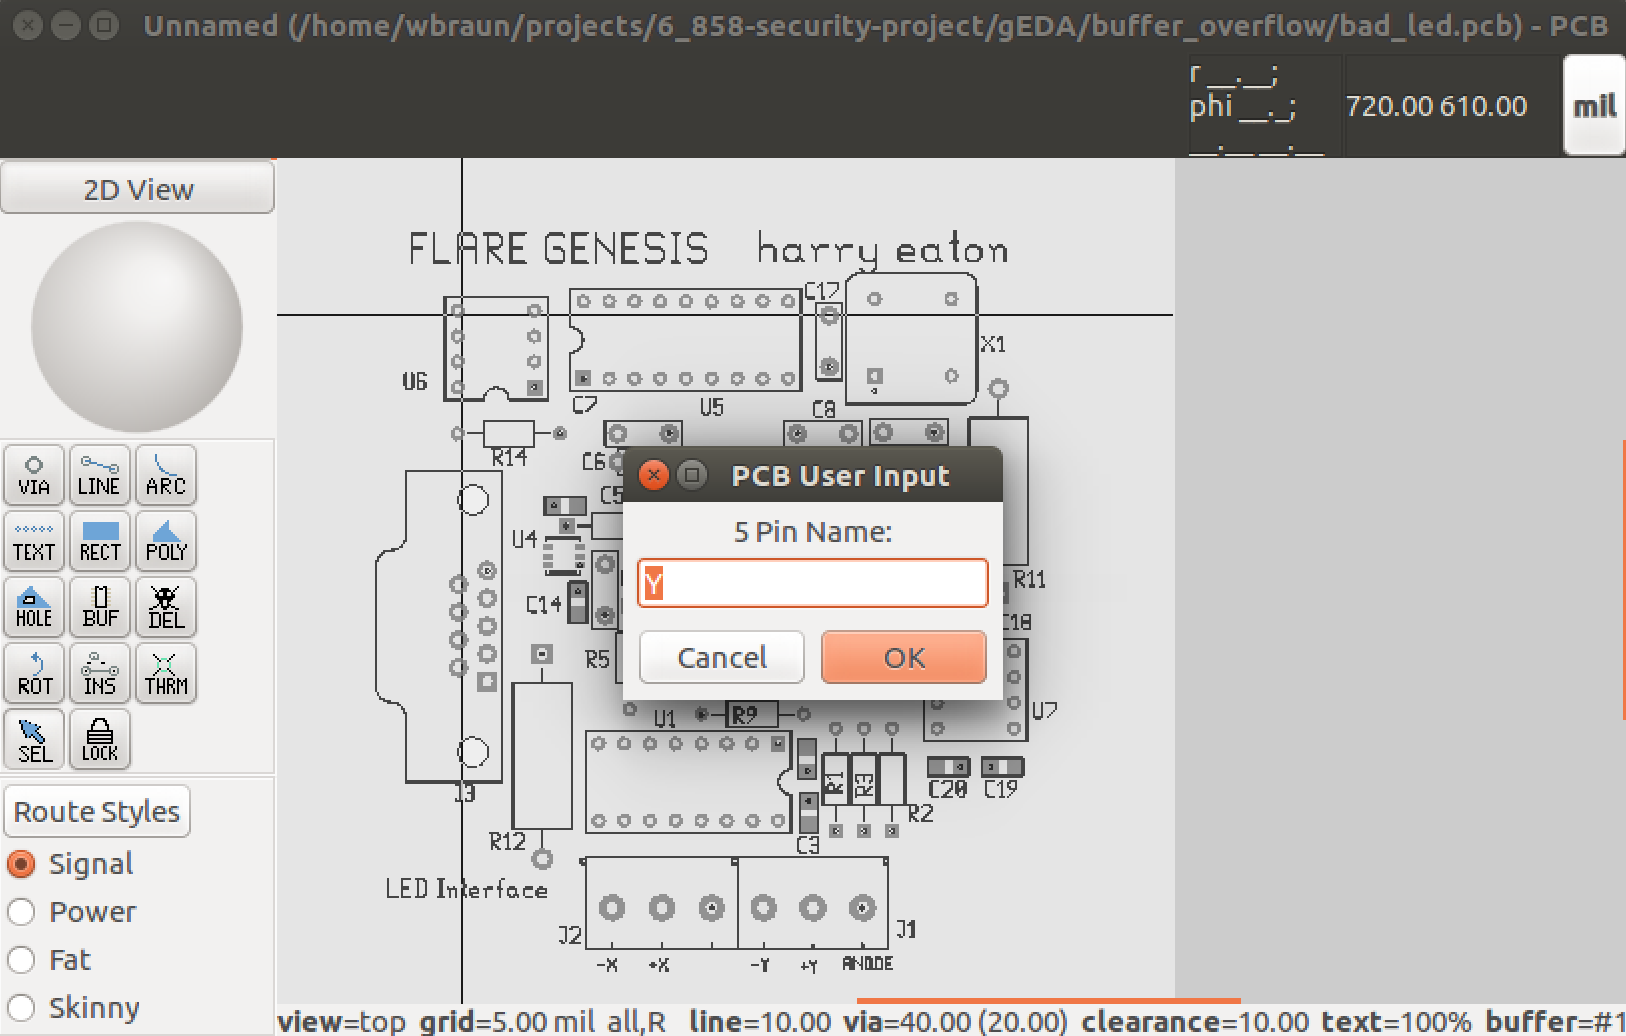
\includegraphics[width=3in]{images/rename-gui.png}
\caption{Pin Renaming Dialog Box}
\label{fig:rename-gui}
\end{figure}

The exploit runs with the address space randomization disabled, stack canaries disabled, fortify source disabled, and stack execution enabled. It would have also been possible to produce a version which did not require an executable stack and instead by redirecting the program control flow to call libc functions. To bypass address space randomization an address leakage would be needed which was not found in the code analysis or fuzzing. 

To produce the exploit file a python script was created that inserts the shellcode, execution address, and padding, in place of the pin number of a chosen pin in an example pcb layout. Once the user opens this file and attempts to rename that pin the shellcode will be executed. Due to the presence of non display characters in the shellcode the payload fails to display via the GUI, hiding the attack from the user. Figure \ref{fig:exploit-gui} shows the pin renaming dialog when the exploit is underway. The example shellcode used for this exploit is borrowed from the 6.858 course material and launches a shell, but could in practice be any malicious action. 

\begin{figure}[H]
\centering
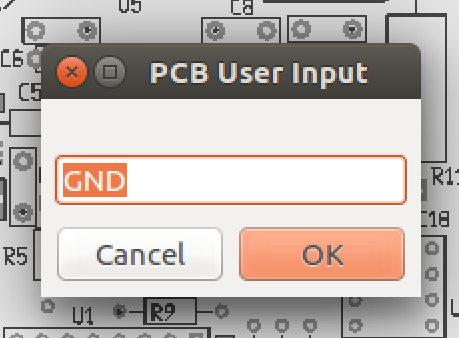
\includegraphics[width=3in]{images/exploit-gui-cropped.png}
\caption{Dialog Box During Exploit}
\label{fig:exploit-gui}
\end{figure}

\section{Future Work}
\label{S:6}
Future work for this project would include writing replacement functions for the GUI library to allow for faster fuzzing and work on utilities to better process the results of the fuzzing. Due to time constraints it was only possible to go though a subset of the unique crashes produced via fuzzing. Having to run GDB and possibly Valgrind for each crash file and manually review the code to discover the cause was extremely time consuming. It may be difficult to automate the process of judging the utility of a vulnerability but even some basic classification would save time. It is highly likely that promising vulnerabilities were missed in the sheer volume of unique crashes. 

\section{Conclusion}
\label{S:7}
Although this project did not result in an exploit which works on an EDA program installed directly from the release website or package manager it did demonstrate the validity of the threat model presented by the sharing of open source hardware design files. Given that the vulnerabilities found were mitigated only by toolchain and OS protections it is quite likely further analysis could find a fully exploitable vulnerability. Additionally, given that the gEDA project dates back to 1998 it is possible that the exploit that was created would have worked on some past computer. The author will sure to be careful in opening any CAD or EDA files sourced from the internet in the future. 

\section{Resources}
\subsection{Project Github Page}
\url{https://github.com/westonb/6_858-security-project}

\subsection{Useful Webpages}
\label{S:8}
\begin{enumerate}
	\item \url{http://www.geda-project.org/} 
	\item \url{http://kicad-pcb.org/}
	\item \url{http://jblevins.org/log/valgrind}
	\item \url{https://fuzzing-project.org/tutorial3.html}
\end{enumerate}

\end{document}